% CVPR 2022 Paper Template
% based on the CVPR template provided by Ming-Ming Cheng (https://github.com/MCG-NKU/CVPR_Template)
% modified and extended by Stefan Roth (stefan.roth@NOSPAMtu-darmstadt.de)

\documentclass[10pt,twocolumn,letterpaper]{article}

%%%%%%%%% PAPER TYPE  - PLEASE UPDATE FOR FINAL VERSION
%\usepackage[review]{cvpr}      % To produce the REVIEW version
%\usepackage{cvpr}              % To produce the CAMERA-READY version
\usepackage[pagenumbers]{cvpr} % To force page numbers, e.g. for an arXiv version

% Include other packages here, before hyperref.
\usepackage{graphicx}
\usepackage{amsmath}
\usepackage{amssymb}
\usepackage{pifont}
\usepackage{booktabs}
\usepackage{multirow}
\usepackage{url}

\newcommand{\aca}[1]{{\color{red}#1}}

% It is strongly recommended to use hyperref, especially for the review version.
% hyperref with option pagebackref eases the reviewers' job.
% Please disable hyperref *only* if you encounter grave issues, e.g. with the
% file validation for the camera-ready version.
%
% If you comment hyperref and then uncomment it, you should delete
% ReviewTempalte.aux before re-running LaTeX.
% (Or just hit 'q' on the first LaTeX run, let it finish, and you
%  should be clear).
\usepackage[pagebackref,breaklinks,colorlinks]{hyperref}


% Support for easy cross-referencing
\usepackage[capitalize]{cleveref}
\crefname{section}{Sec.}{Secs.}
\Crefname{section}{Section}{Sections}
\Crefname{table}{Table}{Tables}
\crefname{table}{Tab.}{Tabs.}


%%%%%%%%% PAPER ID  - PLEASE UPDATE
\def\cvprPaperID{*****} % *** Enter the CVPR Paper ID here
\def\confName{CVPR}
\def\confYear{2022}


\begin{document}

%%%%%%%%% TITLE - PLEASE UPDATE
\title{Attck Monocular Depth Estimation Model with a Sticker}

% \author{First Author\\
% Institution1\\
% Institution1 address\\
% {\tt\small firstauthor@i1.org}
% % For a paper whose authors are all at the same institution,
% % omit the following lines up until the closing ``}''.
% % Additional authors and addresses can be added with ``\and'',
% % just like the second author.
% % To save space, use either the email address or home page, not both
% \and
% Second Author\\
% Institution2\\
% First line of institution2 address\\
% {\tt\small secondauthor@i2.org}
% }
\author{Meng Pan, Fangjun Huang$^\dagger$\\
 School of Computer Science and Engineering, 
Sun Yat-sen University, China\\
{\tt\small panm9@mail2.sysu.edu.cn, huangfj@mail.sysu.edu.cn
}}
\maketitle
\def\thefootnote{$\dagger$}\footnotetext{
	Corresponding author}\def\thefootnote{\arabic{footnote}}

%%%%%%%%% ABSTRACT
\begin{abstract}
	DNNs have been demonstrated that their performance 
	can be degraded by imperceptible perturbations. 
	Monocular Depth Estimation networks with 
	DNNs likewise encounter such a dilemma. 
	This attack diagram, adding perturbations, 
	is not implementable and capturable for a sensor, 
	which means it is an ideal attack diagram. 
	An implementable and applicable attack diagram in 
	the physical world is needed. To this end, we 
	address this by sticking patches into indoor scenes. 
	We proposed an automatic searching and 
	transformation method. In the searching phase, 
	the patch is dispatched to an appropriate and 
	sensitive location exploiting the MDE's gradient. 
	In the transformation phase, the patch alternates 
	its appearance according to its location. 
	In doing this, we can generate destructive, 
	inconspicuous adversarial examples. 
	This whole process doesn't rely on any generate
	networks, which makes it fast and light.
	We evaluate our method on NYU depth v2, 
	experiments show that our method 
	eliminates 6\% of RMSE in 0.8s 
	meanwhile 
	keeping remarkable inconspicuousness.
\end{abstract}

\section{Introduction}
Monocular Depth Estimation~(MDE) algorithms 
is a crucial 3D scene perception method. 
With the rapid development of 
Deep Neural Networks(DNNs), many excellent MDE methods 
base on DNNs have been proposed recently. 
However, according to Szegedy's 
research~\cite{Szegedy_2014_ICLR}, DNNs are 
prone to be attacked by adversarial examples: 
when an imperceptible 
small perturbation is added to an input image, the classifier 
based on DNNs will classify the obtained image, knowned as
adversarial examples, into a wrong category with high probability. 
Adversarial examples have been found not only on classification tasks 
but also on logical regression tasks, such as 
semantic segmentation and 
object recognition. MDE also fail to get rid of this dilemma.
As learned perception modules are increasingly
deployed on autonomous driving vehicles, 
mistaking a stop sign for a speed limit or causing
obstacles to disappear can cause immense damage.
So as a kind of 3D scene perception solution, MDE 
algorithms need to be 
robust and reliable.

%so that when an attack occurs in automatic 
%driving, the vehicle can still accurately perceive the depth 
%of the scene. 
The threat of adverserial example on MDE algorithms was 
first studied by Wong~\textit{et al}~\cite{Wong_2020_NIPS}. 
They conducted 
comprehensive and rigorous experiments to explore the impact 
of pixel attacks on MDE. Including attacking the whole 
depth map of a scene, attacking the depth map of one 
single object in the scene, and even making a specific 
object vanished completely on the depth map by 
adding perturbations. This research is pioneering and 
enlightening for attacking MDE.

\begin{figure}
	\hspace{-0.5cm}
	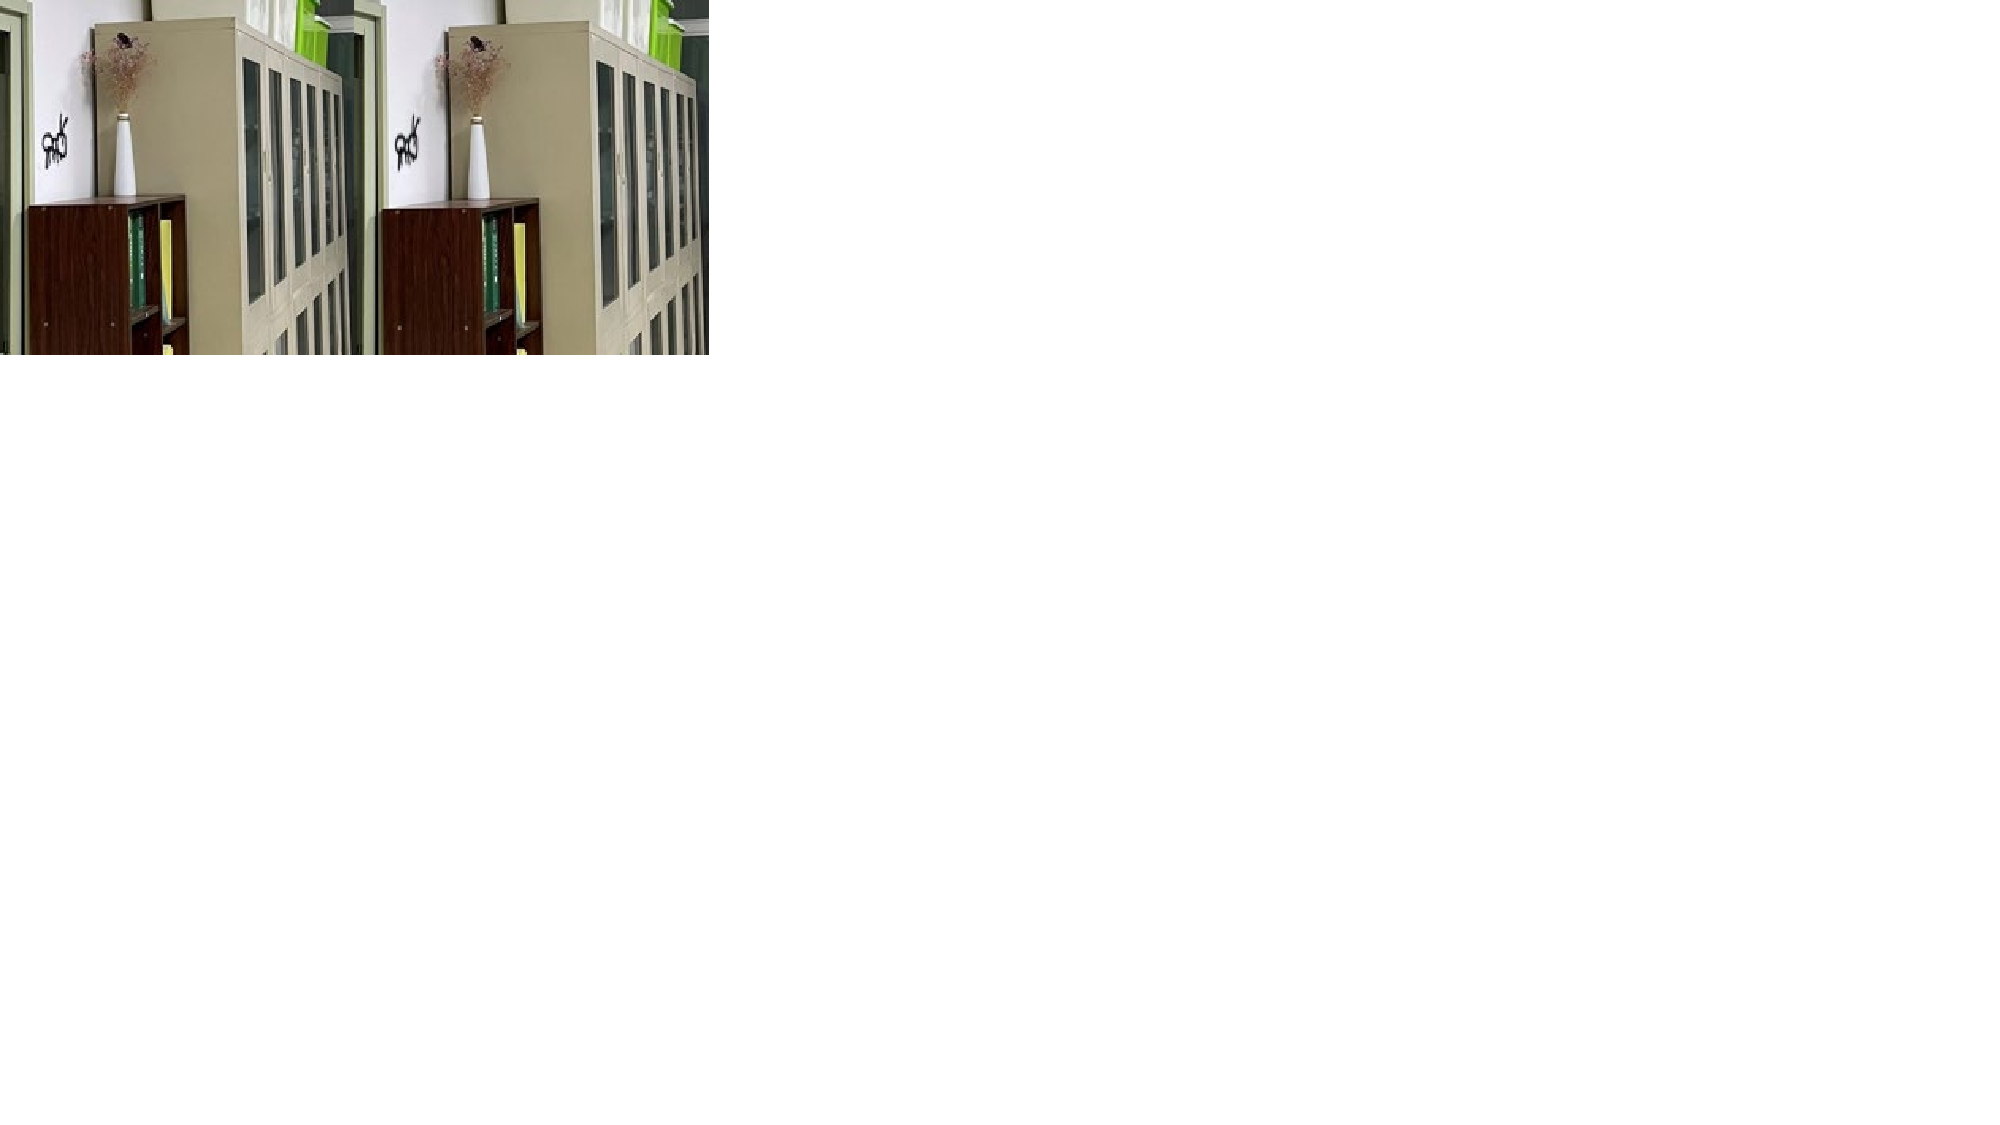
\includegraphics[width=0.5\textwidth]{imgs/preview.pdf}
	\caption{Preview of our patch attack method. 
	The adversarial example generated by our concealed
	attack method(a). 
	We stick a printed draw in physical world~(b), and
	Note that this was shot in our office, 
	not the dataset scene we used in the experiment part.
	}
	\label[]{effect}
\end{figure}
However, the study of Wong~\textit{et al} is hard to be realized
in the physical world, since
the perturbations added on the input images can not 
be perceived by a camera. 
However, attacking scenes with patches is an appropriate solution. 
Camouflaging a patch to a sticker and sticking it 
into the target scene is inconspicuous and easy
to be implemented.

There exist some works exploiting patches to generate 
adversarial examples on image classification,
traffic sign recognition and other tasks.
For example, Brown~\textit{et al}~\cite{Brown_2017_arxiv}
exploited patches to attack 
DNNs, but they didn’t 
pay much attention on inconspicuousness, that is, 
the abrupt and unreal patch in scenes will reveal 
the attack intention.
Later works~\cite{Hu_2021_ICCV,Kong_2020_CVPR,Liu_2019_AAAI}
noticed this problem and utilize 
GAN to make patches
more naturalistic. 
But this will increase time and space complexity obviously.

In this paper, we take physical realizability and 
inconspicuousness into accout, and design a fast and automatic
method to attack MDE algorithms.
Fig.~\ref{effect} shows the rough outline of our method.
Meanwhile it indicate that our adversarial examples generated
on pixel level can be simulated through sticking a printed patch 
on the real scene.

The contributions of this work are as follows:
\begin{itemize}
	\item We are the first to apply patch attack on MDE
	tasks.
	\item We propose a fast, automatic, inconspicuous attack 
	method. In this method, a learnable 
	matrix is designed to update the patch's location. 
	The updating of the location is based on
	attack effect and visual quality using gradient 
	descent automatically. Finally we use perspective 
	transform to alter the patch's appearance and make 
	it looks like a sticker. 
	\item experiments
	show that our method generate destructive while 
    concealed adversarial examples.
\end{itemize}.

The structure in the rest paper is organized as
follows. After a review of MDE and patch attacks in
Sec.~\ref{Background}, we introduce our method 
concretely in Sec.~\ref{Method}. Then we visualize 
the effct of our location searching phase and attack a
MDE network in Sec.~\ref{Experiments}. Finally We
analyze our patch attack method in Sec.~\ref{Conclusion}.


\section{Background}
\label[]{Background}
In this paper, patch attack for MDE model is concentrated on. 
We will give a brief introduction for MDE task and review
the related patch attack works. 
Note that we are the first to attack MDE model with patches,
so the related works only involved image classification,
traffic sign recognition, face recognition, etc. 
But these works still inspire us a lot.

\subsection{Monocular Depth Estimation}
\label[]{MDE}
\begin{figure}
	\centering
	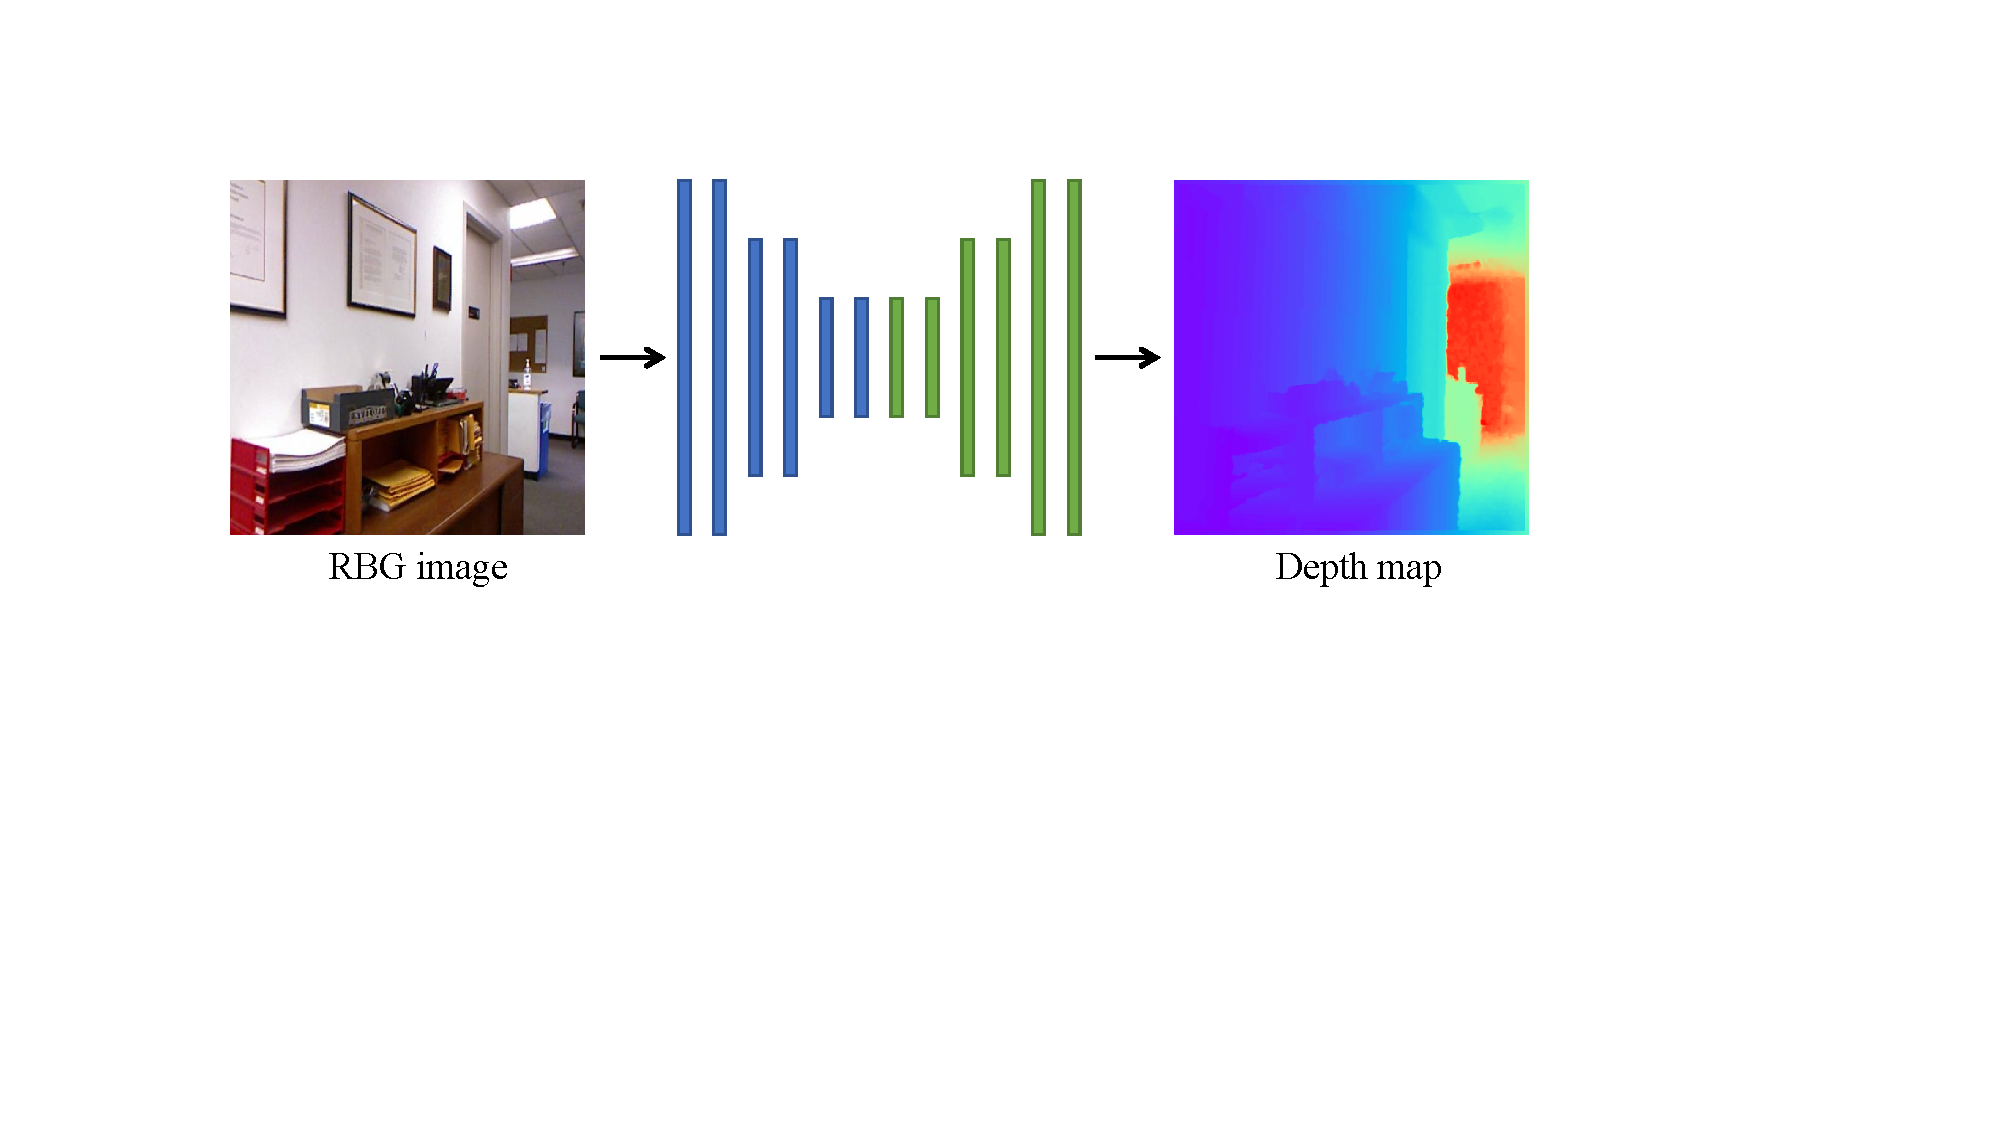
\includegraphics[width=1\linewidth]{imgs/MDE.pdf}
	\caption{A common stream of MDE algorithm.}
	\label[]{stream of mde}
\end{figure}
MDE algorithms can generate dense depth map for each pixel in 
the given RGB image.
They achieve satisfactory results base on advanced DNNs. 
Fig.~\ref{stream of mde} shows a common inference stream of MDE model:
A RGB image is fed into the MDE model, which generate dense 
depth map for the image. The training of the model needs
immense, dense annotated images and depth maps.
However, suffered from the lack of sufficient geometric constraints, 
MDE is still an ill-posed problem. 
%\subsubsection{Supervised}
%DNNs learn through the supervision of ground truth labels 
%annotated artificially. Since the mapping from a single image 
%to a depth map is very complicated, this supervised learning 
%manner is very suitable for MDE tasks. The initial work adopts 
%this \textbf{intuitive endoder-decoder} concept. 
%Eigen et al.~\cite{Eigen_2014_nips} designed two hierarchical 
%neural networks to predict 
%the depth map in coarse and fine respectively.
%A network was proposed subsequently by them~\cite{Eigen_2015_ICCV}, 
%in which three 
%different tasks, depth estimation, segmentation and 
%normals prediction was integrated into one model.
%Lee~\cite{lee_2019_arxiv} coined novel local planar 
%guidance layers and locate 
%them at different scale decoding phases. 
%As a result of this, final fine depth maps are densely 
%restored from small to big.
In this paper, to study the effect of patch adversarial examples, 
we examine the robustness of Fastdepth~\cite{Wofk_2019_ICRA}, an
efficient and lightweight encoder-decoder MDE network.
%Some researches~\cite{Li_2018_ACCV,cao_2017_CSVT,Fu_2018_CVPR} 
%address this problem by formulizing it as 
%a \textbf{classification} problem. 
%Discrete depth labels are prepared by separating 
%continuous depth value, which are then used to supervise 
%the training process.
%While using \textbf{relative depth information} to predict depth 
%indirectly is also a effective solution.
%Lee~\cite{Lee_2019_CVPR} proposed a method to predict depth from relative depth. 
%They first estimate relative depth by utilizing rank-1 property, 
%then the final depth maps are reconstructed through these relative 
%depth maps.

\begin{figure*}[htb]
	\centering
	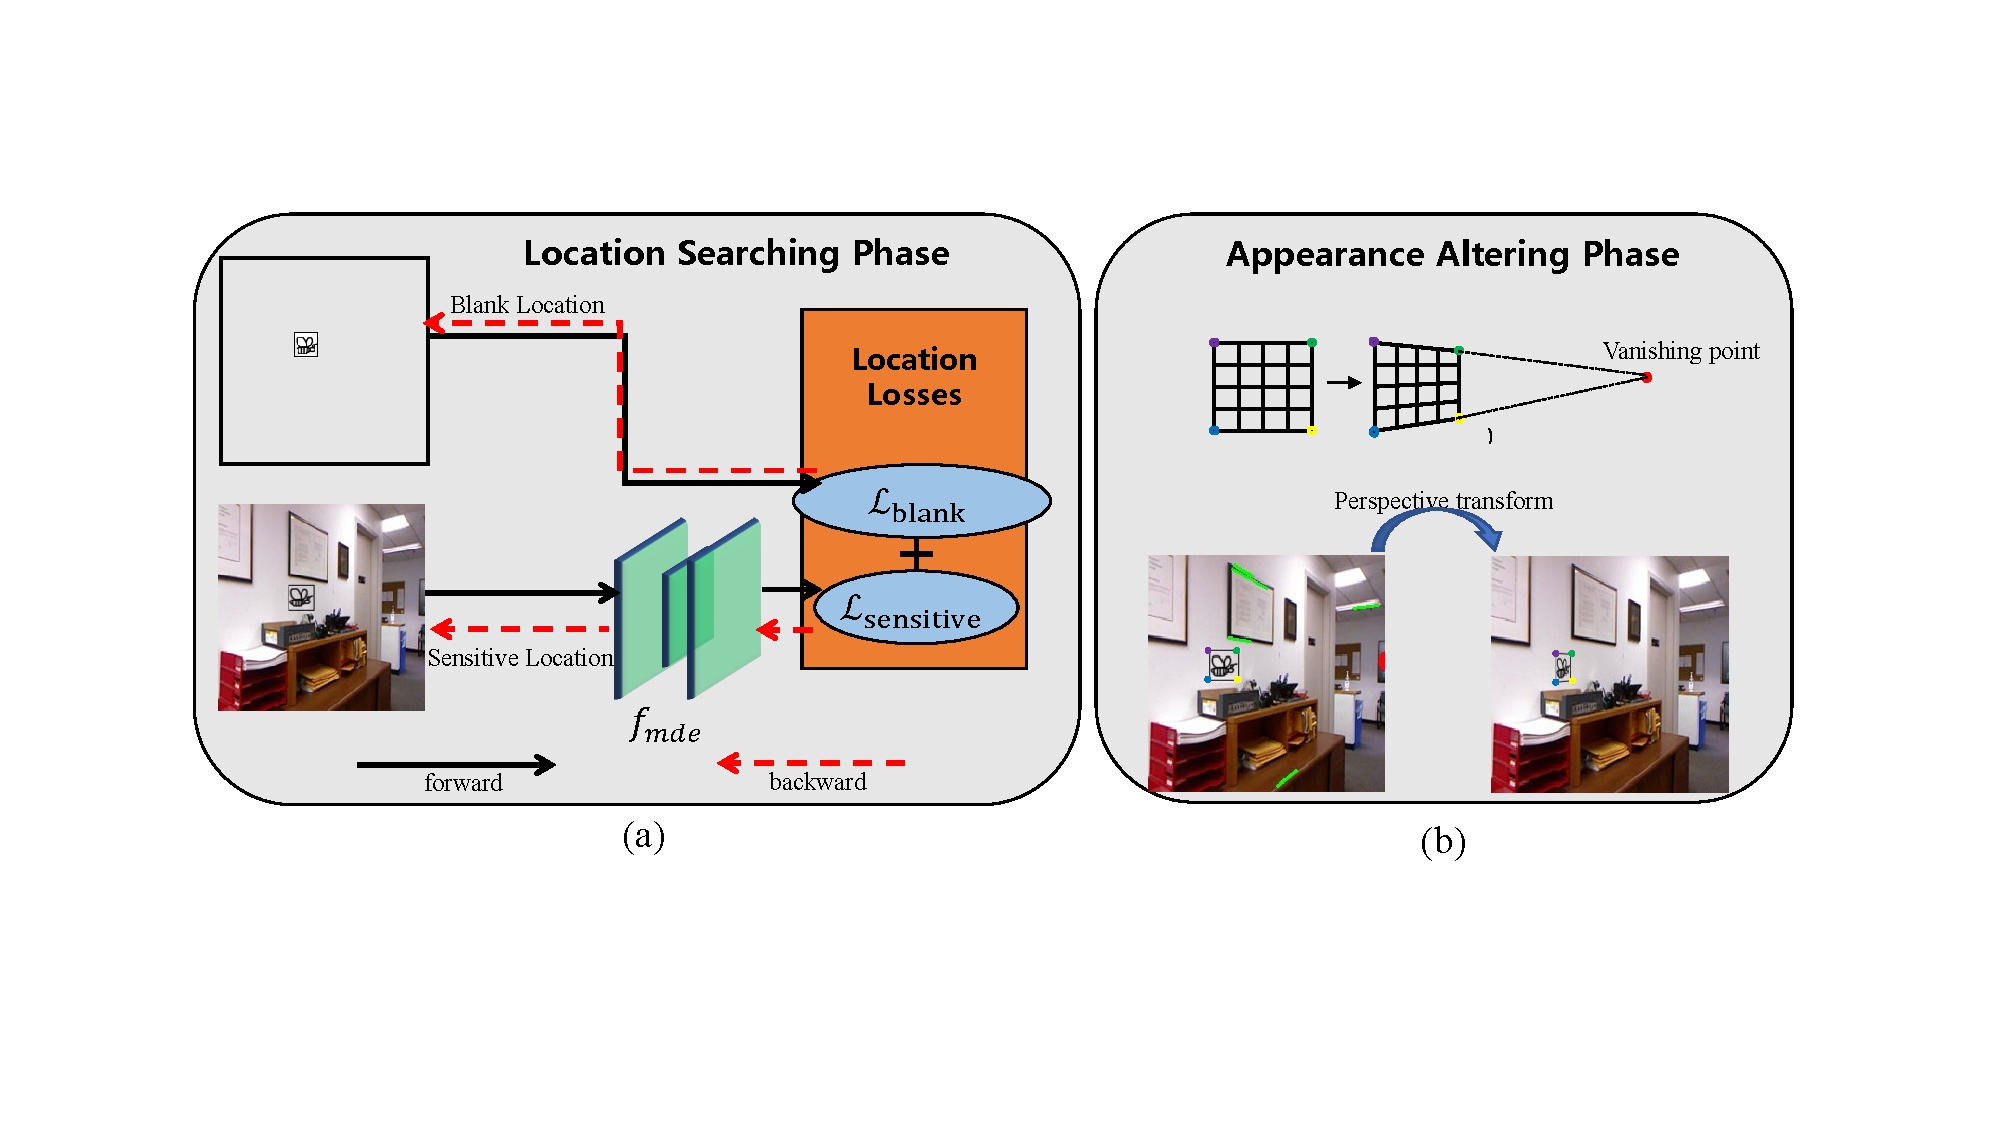
\includegraphics[width=1\textwidth]{imgs/stream.pdf}
	\caption{Stream of our MDE attacking method. 
	The whole stream consists of two phases: (a) location
	searching phase and (b) altering appearance phase. They
	are described concretely in Sec.~\ref{Location Searching}
	and Sec.~\ref{Appearance Altering}}
	\label[]{stream}
\end{figure*}
%\subsubsection{Unsupervised}
%Although there exist some datasets with ground truth depth 
%annotation, dense and accurate depth maps are labor-consuming and rare. 
%In that case, unsupervised methods dominate recently.
%Godard et al.~\cite{Godard_2017_CVPR} exploit the left-right 
%consistency of binocular image pairs
%to tackle this issue: 
%with a decently predicted disparity, 
%the two images sampled from a binocular camera can 
%synthesize each other. 
%A consecutive vedio sequence can provide a constrain for MDE.
%Given a middle frame and its former, later frame sampled from a video, 
%DNNs can estimate the camera pose and the depth, with which we can 
%restore the other two frames. Based on this constrain, camera pose 
%and depth can be learned jointly~\cite{Zhou_2017_CVPR}.
%However, there is a flaw in both video and binocular solutions.
%On the one hand, binocular image pairs methods struggle in occlusion 
%and texture-copy problems, yet, on the other hand, as an 
%alternative method, 
%predicting depth from a video performs unsatisfactorily 
%when it comes to relatively stationary objects.
%To address this, Godard et al.~\cite{Godard_2019_ICCV} 
%proposed a multi-scale reconstruction
%loss and a automasking approach to ignore relatively stationary objects.
\subsection{Patch Attack}
Adding perturbations to images has a limit: 
the imperceptive noise can not be captured by camera.
Recently, researchers turn to generating adversarial examples with
patches. It can be captured by camera and it can implement to physical
world. The only question is, how to make it concealed.

Sharif et al.~\cite{Sharif_2017_CCS} attacked FRS using real 
printed glass frames, 
with which the FRS can not recognize the person or recognize him
as someone else in the system. The pattern of these frames are 
generated by optimizing a composite objective function, 
including gradient decenting, smoothness of perturbations and 
non-printability score (NPS) optimal terms.
Tom et al.~\cite{Brown_2017_arxiv} abandon the camouflage of the attack, 
they attack DNNs with an apparent, universal patch, 
which is updated with different locations and transformations settings.
To generate robust adversaries, 
eykholt et al.~\cite{Eykholt_2018_CVPR} sampled from both 
actual physical and synthetic transformation images. Besides,
they found that there exist vulnerable and robust areas in an 
image and identified these areas by computing perturbations 
using the $L_1$ regularization. Then they generate perturbations 
using $L_2$ regularization on vulnerable areas, finally reshape 
the perturbations to a graffiti shape. In doing so, they achieve 
a high successful rate under various environmental conditions.
Liu et al.~\cite{Liu_2019_AAAI} also attacked the traffic signs. 
Instead of 
locating the vulnerable areas by computing, they locate 
the patch by a attention model, which takes as input the 
traffic sign, outputs an mask that indicates where to put the patch. 
The patch is generated through a GAN, which consists of a generator 
to generate a misclassification patch and a discriminator 
to discriminate whether the patch is original or adversarial. 
Kong et al.~\cite{Kong_2020_CVPR} also use a GAN to generate 
perturbation patches. 
In particular, they manipulate advertisement posters as original patch, 
which is artificially stuck on a street billboard after it 
through a GAN. This method produces better inconspicuousness yet 
the process of sticking the patch to billboard is labor consuming.
%The location of a patch matters to the camouflage. 
In~\cite{Hu_2021_ICCV}, the locations of patches are artificially 
determined and fixed
to make a better camouflage.
They first detect all humans in an image and pin a generated patch 
on their shirt. This attack makes the adversarial examples look as 
natural as a natural shirt pattern.
Forwardmentioned attack methods need to access to the objects they 
attacked. The advantage is that adversarial examples are more 
inconspicuous, it is hard to deployment in the physical world though. 
To this end, Zolfi et al.~\cite{Zolfi_2021_CVPR} proposed 
a contactless attack method. 
Several translucent patches are generated by updating the affine 
transformation matrix, then they are deployed on the camera's lens.

\section{Method}
\label[]{Method}
In this section, our MDE attacking method 
is presentd in detail. we first formulize the problem 
as an optimal problem
in Sec.~\ref{Problem Statement}. 
Then we describe how we design our patch, the objective
function and how the patches are optimized 
in Sec.~\ref{Location Searching}. 
Finally the appearance altering phase is introduced in
Sec.~\ref{Appearance Altering}.

\subsection{Problem Statement}
\label[]{Problem Statement}
As stated in Sec.~\ref{MDE}, the problem of predicting
a depth map from a single RGB image can be treated as
a supervised learning problem.
Denoting as $\mathcal{I}$ the space
of RGB images and as $\mathcal{D}$ the domain of annotated depth
maps, given a training set 
$\mathcal{T}={(I^{H \times W \times 3}, D^{H \times W \times})}$, 
$I \in \mathcal{I}$ and $D \in \mathcal{D}$, 
a MDE model $f_{mde}$ can learning a non-linear mapping
$f_{mde}: \mathcal{I}\rightarrow \mathcal{D}$.
%We denote by 
%$f_{mde}:\mathbb{R}^{H \times W \times 3}\rightarrow
%\mathbb{R}^{H \times W}$ a MDE model.
Considering elaborately designed 
perturbations can hardly be obtained by consumer cameras, 
Our adversarial examples are generated through sticking 
patches $\delta$ on appropriate areas. 
Here we use following simplified equation denote our
adversarial examples.
Specific expression can be found in Sec.~\ref{Patch Design}.
\begin{align}
	I^{adv} = I + \delta 
\end{align}
%Note that this is 
%a representation of attacking with one patch, 
%we adopt more than one patch in our 
%following experiments. 
Our goal, attacking a MDE model, is to 
maximize the error of ground truth depth map $D^{*}$ and 
depth map generated from $I^{adv}$.
\begin{align}
	\max  \Vert f_{mde}(I^{adv}) - D^{*} \Vert_{p}
\end{align} 
$\Vert \centerdot \Vert_p$ denotes the $l_p$ norm.
%Different with former works, we do not use patches generated by 
%adding perturbations or through a GAN, we simply use a 
%perspective transformation matrix $T$ to update the location and 
%shape of the patch to make it 
%more destructive, more concealed, meanwhile, save 
%more optimization time.
%Our final definition of the adversarial examples is:
%\begin{align}
%	I^{'} = (1 - m) \odot I + T\delta 
%\end{align}

\subsection{Location Searching}
\label[]{Location Searching}

In this subsection we are goint to 
explicate our location searching phase.
Including patch design, our objective function
and optimization of the location.
The stream of the location searching phase can be seen in 
Fig~\ref{stream}(a). 
%Current works leverage a GAN to add perturbations on patterns or 
%generate patterns, which has more time and spatial complexity. 
%In this section, we will introduce our fast and light optimal 
%method in detail, which searches the most destructive area and 
%transforms the patches to a more rational style before sticking.
\subsubsection{Patch Design}
\label[]{Patch Design}
We hope the patch stuck in the scene looks like graffiti,
so a simple line-drawn patch is preferred.
Therefore, a patch is selected from QuickDraw~\cite{quickdraw},
a collection of 50 million hand-writing drawings across 345 categories.
to generate our adversarial examples $I^{adv}$.

To obtain $I^{adv}$,
the first problem we encountered is where to stick the patches.
Exhaustive search is feasible but time consuming. We expect to
complete this process automatically and quickly.
So we turn to optimizing the patch location 
by gradient decenting.  
To this end, A mask $M$ is defined to realize the 
movement of the patch:
we place the patch $\delta$ in the center of the 
clean image $I$, then the patch is expanded 
to the size of $I$ by padding one around it.
As you can see from Fig.~\ref{}, the patch is simple line-drawn,
which means there is plenty of white area in it.
Thus, to reduce modifications to $I$, $I^{adv}$ can be represented by:
\begin{align}
	I^{adv} = M \odot I 
\end{align}
The homogeneous coordinate of this 
mask is noted as $G$ and its size is $H\times W\times 3$.
We define a $2 \times 3$ matrix 
$\mathbf{A}_\theta$ for each patch to implement this 
location search process.
By optimizing this $\mathbf{A}_\theta$, a patch can update its 
location automatically.
\begin{align}
	\left[
		\begin{array}{ccc}
			1 & 0 & t_x \\
			0 & 1 & t_y \\
		\end{array}
		\right]      
\end{align}
where $[t_x,t_y]^\top$ denote the offsets $\textbf{T}$ in 
horizontal and vertical directions, respectively. 
Initial values are $[0,0]$, which represent
that the center of the patch is on the center of the image.

\begin{figure}
	\centering
	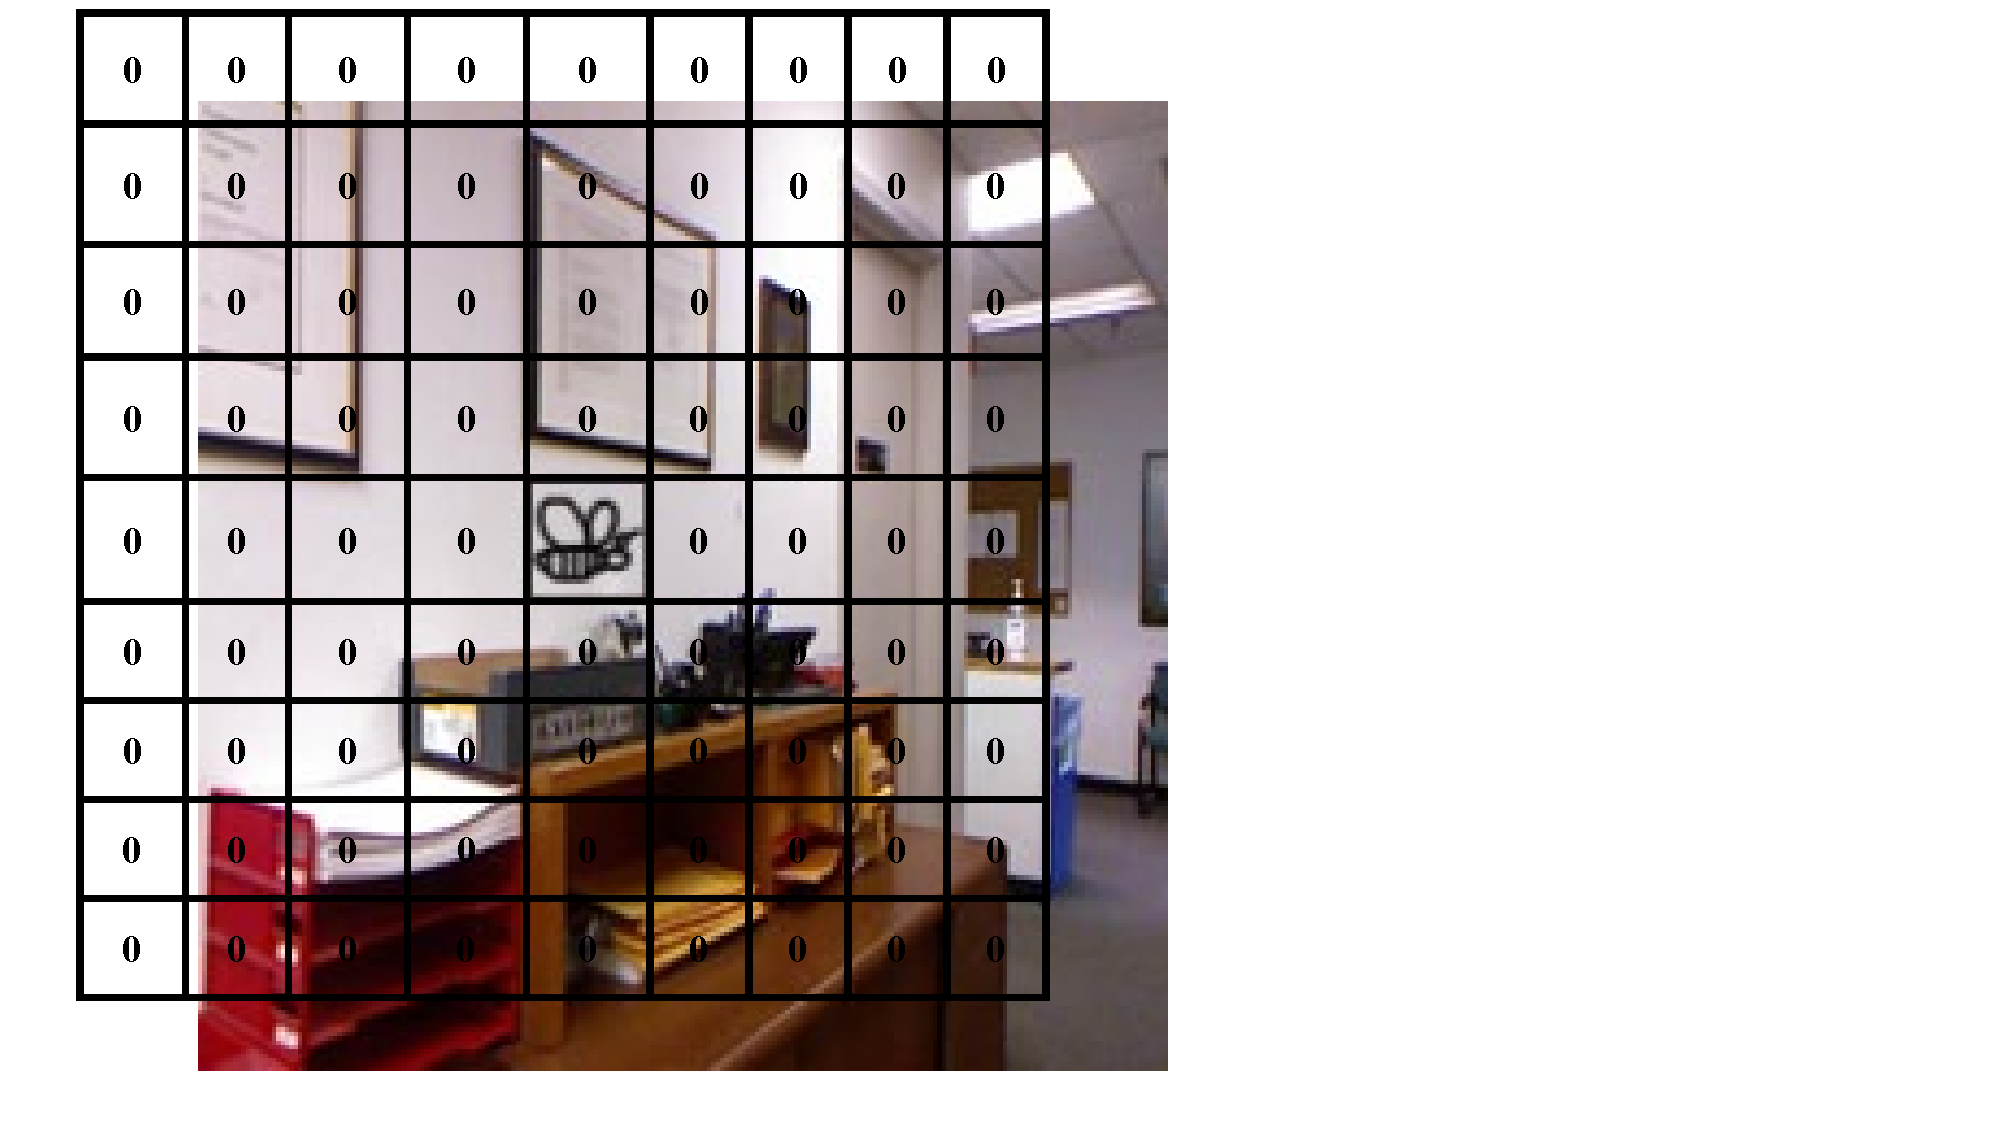
\includegraphics[width=0.4\textwidth]{imgs/mask.pdf}
	\caption{Illustration of our mask $M$, with which
	we can move a patch on images to be attacked through
	$(1 - M) \odot I + \delta$.}
	\label[]{move}
\end{figure}
For each pixel of $m$, $G_i = (x_i, y_i, 1)$.
This movement of the mask can be represented as:
\begin{align}
	{G'}^T = A_{\theta}~{G}^T
\end{align}
\begin{align}
	\label[]{new coordinate}
\begin{pmatrix}
	x_s\\
	y_s	
	\end{pmatrix} = 
		\left[
			\begin{array}{ccc}
				1 & 0 & t_x \\
				0 & 1 & t_y \\
			\end{array}
			\right] 
			\begin{pmatrix}
				x_t\\
				y_t\\
				1	
				\end{pmatrix} 
\end{align}
Finally we got the patch movement on the image 
through moving mask $M$: $(1 - M) \odot I + \delta$.

%$[m,n] \in [-1,1]$ denote the perspective parameters.
%Given a monocular image $I \in \mathbb{R}^{H\times W\times 3}$,
%the pixel coordinates form a grid$H \times W \times 2$.


\subsubsection{Objective Function}
\label[]{Objective Function}
The aim of this research is to attack MDE models inconspicuously 
with patches, we consider three factors: attack effect, 
which area of the adversarial example is more inconspicuous 
and what appearance of the patches are more 
inconspicuous.
The last consideration about the appearance is addressed
by perspective geometry, while the attack effect and 
inconspicuous areas are optimized by two loss funtions
respectively.
The two loss functions consisit 
our objective function in a linear manner:
\begin{equation}
\begin{aligned}
	&\mathcal{L}_{total} = \mathcal{L}_{attack} +
	\mathcal{L}_{blank}\\ 
\end{aligned}
\end{equation}
We are going to explain the two loss functions in the following
part of this section.

\paragraph{attack effect}
MDE models $f_{mde}$ generate depth maps, whose pixel values 
represent the distance from area to sample sensors.
To obtain best attack effect, that is, 
to maximize the error between prediction maps and annotated maps:
\begin{align}
\mathcal{L}_{attack} = \Vert f_{mde}(I^{adv}) - D^{*} \Vert_{p}
\end{align}
We use $L_1, L_2$ and Huber loss in our experiments.

\paragraph{Visualization Quality}
For better inconspicuousness, we camouflage the patch 
as graffiti, which can be usually found on 
blank walls. Blank means with no pictures, marks or 
decoration on white walls.
Based on this we design Blank loss to help the patch to 
find blank areas, the Blank loss
consisits of two optimization sub-terms:
	\begin{align}
		\label[]{blank}
		\mathcal{L}_{blank} = \mathcal{L}_{smooth}+\mathcal{L}_{white}
 	\end{align}
$\mathcal{L}_{smooth}$ constrain the patch locate
on areas with low texture complexity:
	\begin{align}
		\label[]{smooth}
		\mathcal{L}_{smooth} = 
		-\frac{\sqrt{\partial_x (m \odot I) + \partial_y (m \odot I)}}{n} 
 	\end{align}
where $\partial_x$ and $\partial_y$
denote the gradient in $x$ and $y$ directions respectively.
$n$ is the number of pixels in $m$.
$\mathcal{L}_{white}$ constrain the patch locate
 on white areas:
	\begin{align}
		\label[]{white}
		\mathcal{L}_{white} = \frac{\sum_{1}^{n} m \odot I}{n} 
 	\end{align}

\subsubsection{location Optimization}
As indicated in Eq.\ref{new coordinate},
the coordinates of the target pixels $G'_i$ 
are continuous values. 
We adopt bilinear interpolation to determine the value of 
the target pixel. 
Bilinear interpolation mechanism is proved 
to be differentiable in 
\textit{spatial transformer networks}~\cite{stn}.
By maximizing the $\mathcal{L}_{attack}$, 
we can optimize the offsets $\textbf{T}$ step by step.
\begin{align}
    \textbf{T}_0 = [0,0]^\top , \textbf{T}_{S+1} = Clip \{\textbf{T}_{S} + \alpha 
	{\bigtriangledown_{\textbf{T}}\mathcal{L}_{total}}\}. 
	\label[]{optimization}
\end{align}
To avoid patches overflowing from RGB images, $\textbf{T}$ are
clipped between $(-0.875,0.875)$.
For all experiments we set 
$\alpha = 0.004$, 
total optimization step is 50 steps.

\subsection{Appearance Altering}
\label[]{Appearance Altering}
The location problem is settled by optimizing an
affine transform matrix
$\mathbf{A}_\theta$,
next we address altering the appearance of the patch.
The appearance altering phase can be seen in 
Fig~\ref{stream}(b).

\begin{figure}[tb]
	\centering
	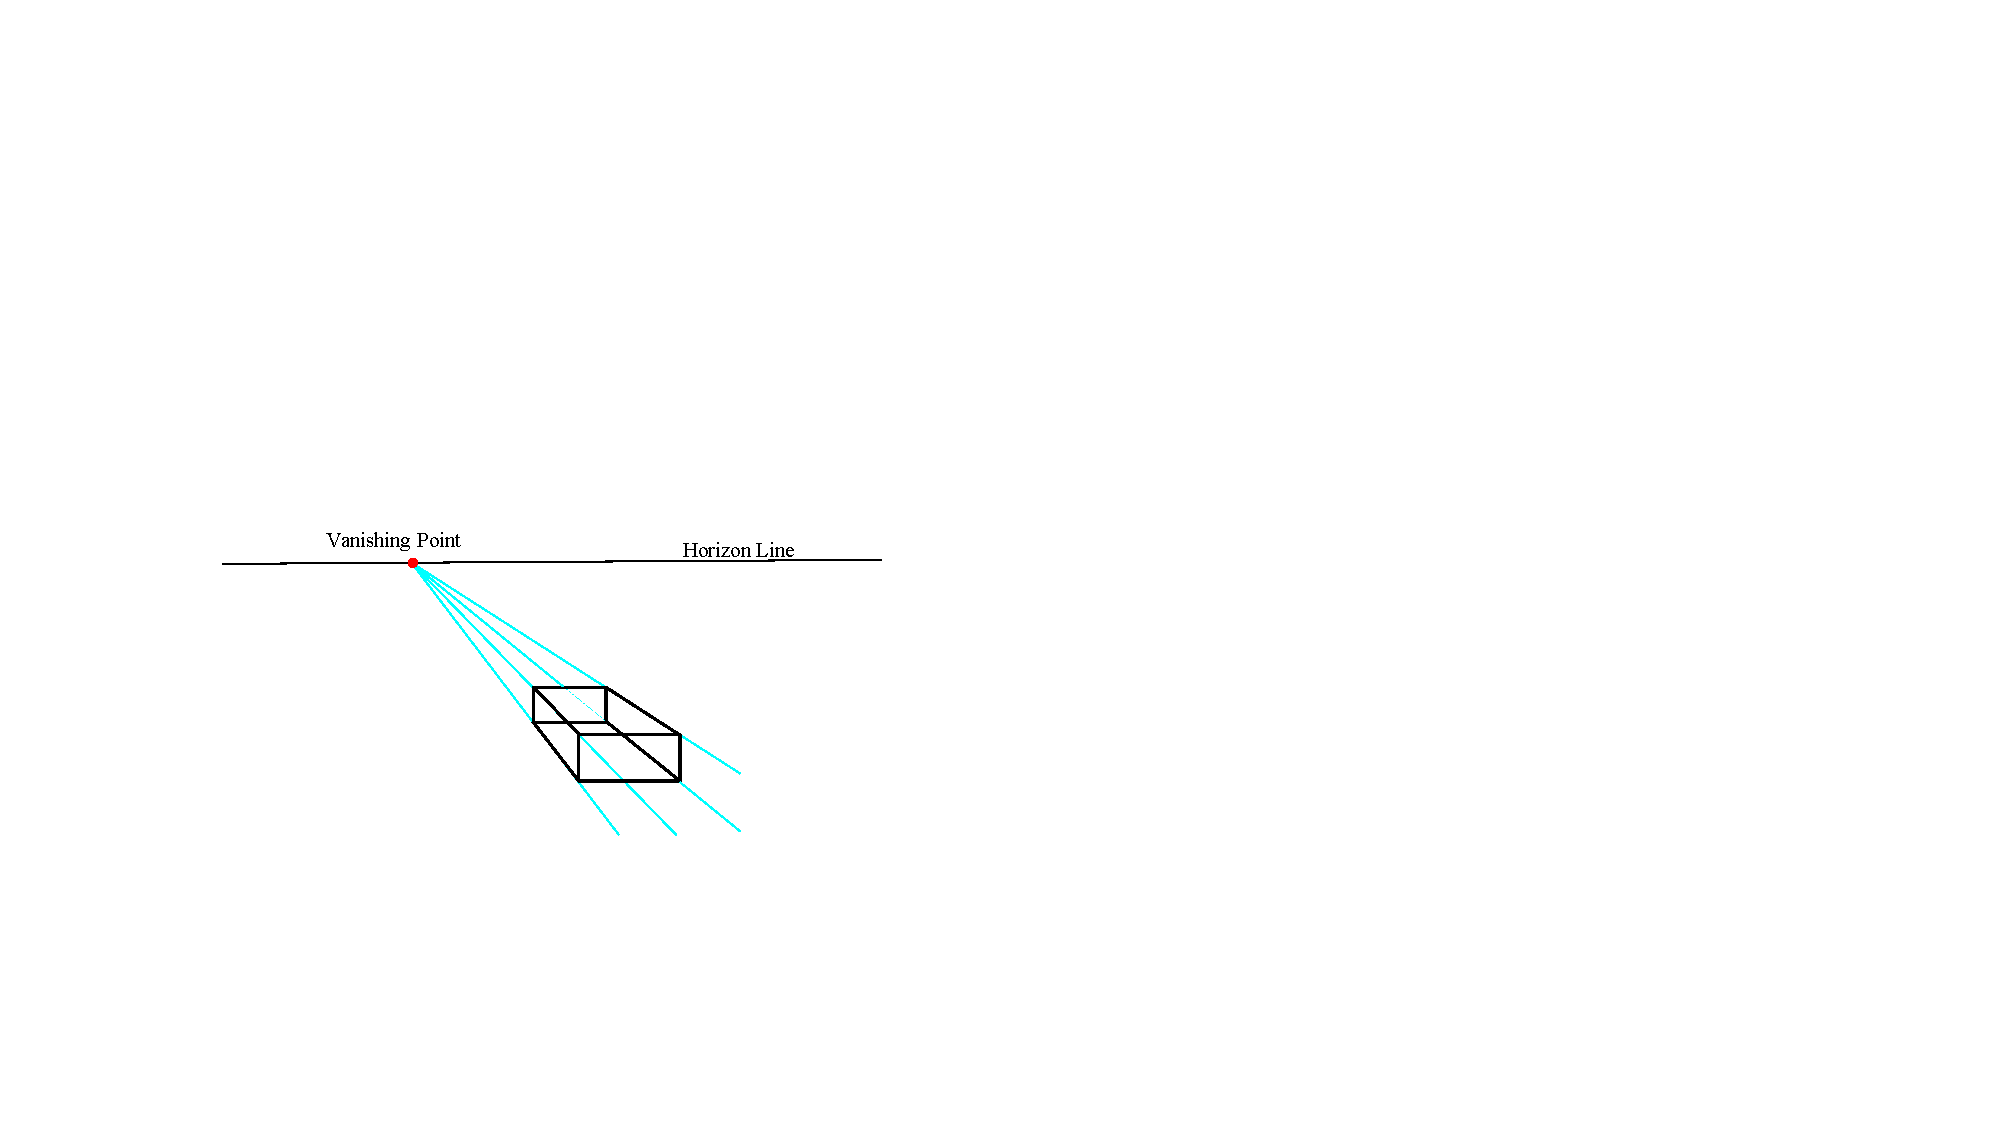
\includegraphics[width=1\linewidth]{imgs/perspective.pdf}	
	\caption{Diagram of single point perspective drawing:
	All the vanishing lines lead to the vanishing point.
	The horizontal and vertical lines, however, 
	remain parallel to each other.}
	\label[]{perspective}
\end{figure}
When we alter the appearance of the patch, 
for better visualization quality, we followed 
the principle of perspective drawing: 
the vanishing point is where all parallel lines 
intersect and is always on the horizon line.
Fig~\ref{perspective} clearly 
illustrates this principle.

We first detect straight lines in the attacked 
scene with \textit{Hough} transform, then we obtain 
the vanishing point by extending this lines 
and computing their intersection.
Based on the principle of perspective drawing, as illustrated
in Fig~\ref{stream}(b), if we connect the left-top point and 
vanishing point, the right-top point should lay on this 
line. Same on the bottom line.
Meanwhile, the connection lines, which converge to vanishing
points, will look shorter than their original length. 
We explain this fact in Fig~\ref{stream}(b):
when seen from the front
view, the width of patches $w$ will shrink to $w'$.
\begin{align}
	w' = \sqrt{w^2-d^2}
\end{align}
Since this task we concentrate on is just MDE, we possess
the depth of each pixel. 
The patches' depth $d$ can be
got by subtracting fronter boarder depth from 
back boarder depth. We set $w=0.1m$ in our experiments.
We get four corrected corner coordinates, with which we 
alter the appearance of the patch. The perspective
transforms in this phase are implemented with 
\textit{OpenCV}. 

\section{Experiments}
\label[]{Experiments}
\begin{figure*}[h]
	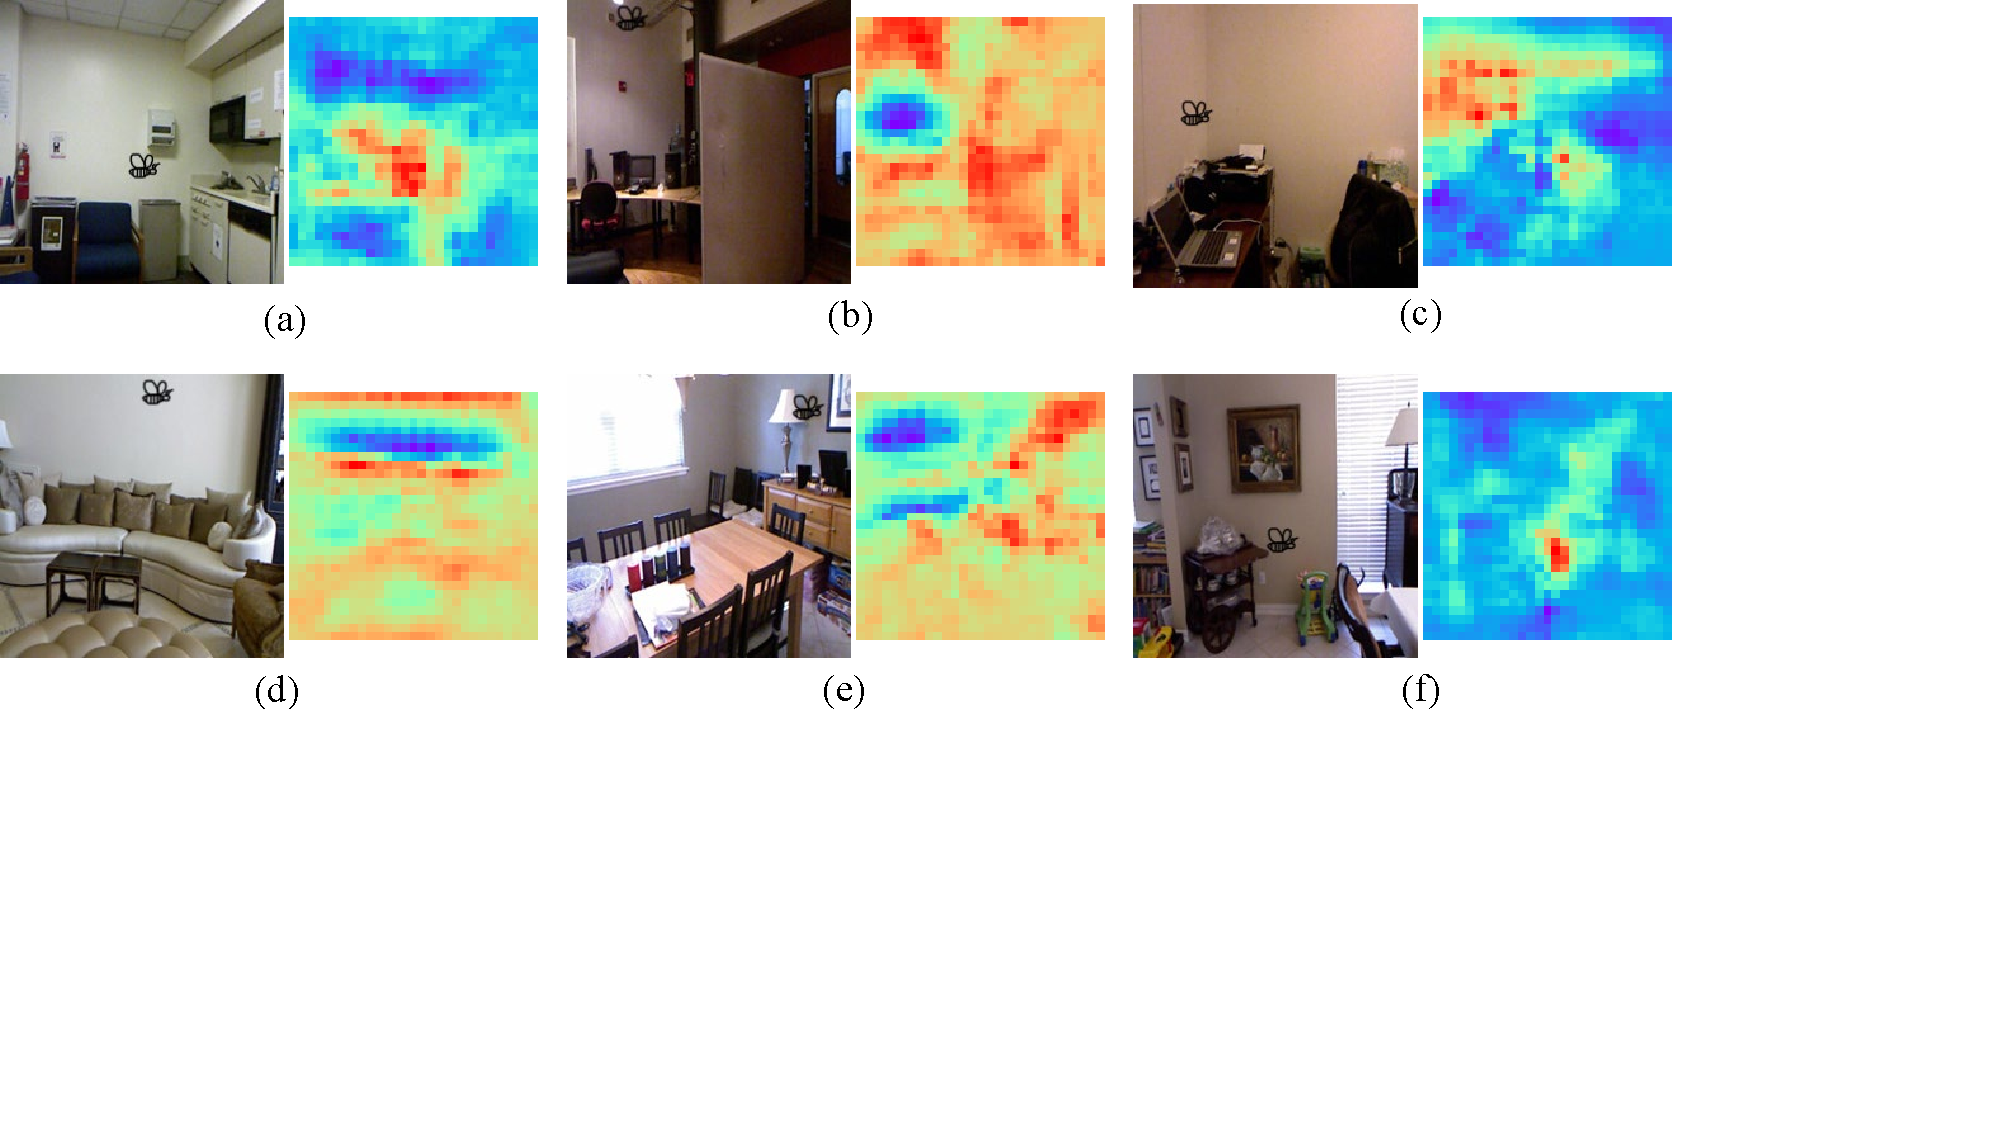
\includegraphics[width=1\textwidth]{imgs/patch_on_scenes.pdf}
	\caption{The final attack locations searched by our method (left) 
	and corresponding MAE maps (right). 
	Then calculate MAE maps, the offsets of the patch 
	are clamped between -0.875 and 0.875, 
	which makes the maps a little smaller than the RGB images.
	}
	\label[]{patch_on_scenes}
\end{figure*}
In this section, we conduct several experiments to exhibit 
the results of our automatic and inconspicuous attack
method on the fastdepth~\cite{Wofk_2019_ICRA} MDE system. 
%As mentioned before, we consider three factors: attack effect, 
%which area of the adversarial example is more inconspicuous 
%and how to make the patches more 
%inconspicuous. 
We introduce our implemention detail, including datasets,
data pre-processing and experiment environment in
Sec.~\ref{Implemention Detail}.
In Sec.~\ref{Visualization Attack Results} and 
Sec.~\ref{Quantitative Attack Results}, 
our attack effects are shown by visualization
and quantitative comparison.
Then we demonstrate the automatic searching process driven 
by our method in Sec.~\ref{Automatic Searching}. Finally we
show and analyze the visual quality of our adversarial examples. 

\begin{figure*}[h]
	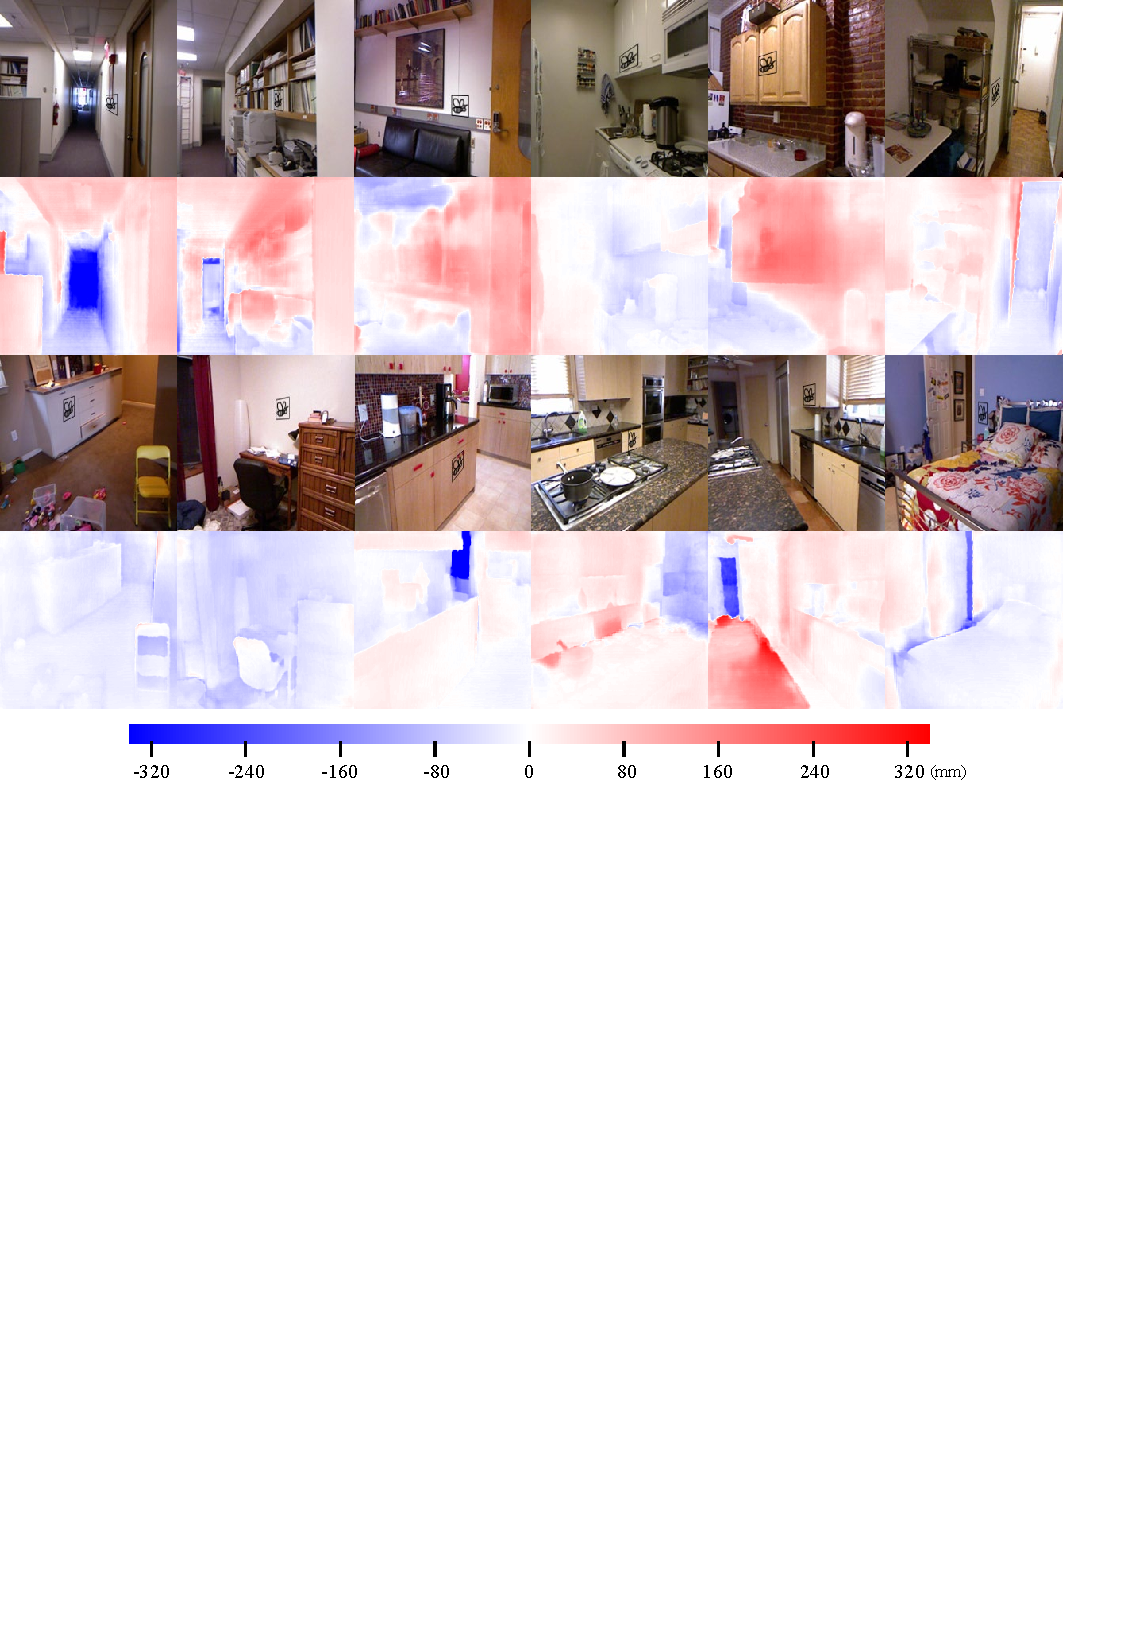
\includegraphics[width=1\textwidth]{imgs/results.pdf}
	\caption{The visualization of our patch attack
	method. The first and third rows are $I^{adv}$.
	The second and fourth rows are the visualization
	of prediction error: 
	$f_{mde}(I^{adv}) - D^{*}$.
	The color bar down the results explicates the 
	error value intuitively.
	We emphasize the patches using surrounding 
	black boxes, which are transformed in the 
	altering appearance phase also.}
	\label[]{results}
\end{figure*}
\subsection{Implemention Detail}
\label[]{Implemention Detail}
For the MDE system, we use Fastdepth~\cite{Wofk_2019_ICRA}. 
We also use the same dataset NYU Depth v2
~\cite{Silberman_2012_ECCV} used in
the Fastdepth~\cite{Wofk_2019_ICRA}. 
This dataset is an indoor dataset, whose depth range is 
0-10 m.
It consisits of 1449 densely annotated depth and RGB images pairs,
795 of which are split to train dataset and the rest are
split to test dataset.
For the image pre-processing, we followed the process in
Fastdepth: images are resize to $250 \times 333$ firstly, 
secondly, center cropped to $224 \times 304$, in the end 
they are resized to $224 \times 224$.

For the patch dataset, we choose QuickDraw~\cite{quickdraw}.
QuickDraw is a collection of 50 
million hand-writing drawings across 345 categories.
We select several categories, including bee, ant,
dolphin, crocodile and so on. The size of them are
all $28 \times 28$.

%®
We focus on four metrics used in previews works to evaluate 
the attack effect: 
\begin{align}
 RMSE=\sqrt{\frac{1}{\lvert N \rvert} \sum\nolimits_{i\in N}\lvert|d_i - d_i^*\rvert|^2} 
\end{align}

\begin{align}
 MAE=\frac{1}{\lvert N \rvert} \sum\nolimits_{i\in N}|d_i - d_i^*| 
\end{align}

\begin{align}
  Abs \ Rel=\frac{1}{\lvert N \rvert}\sum\nolimits_{i \in N}\frac{\lvert d_i - d_i^* \rvert}{d_i^*}
\end{align}

\begin{align}
  Threshold: \% \ of \ d_i \ s.t. \max(\frac{d_i}{d_i^*},\frac{d_i^*}{d_i})=\delta < thr 
\end{align}
$thr$ denotes three threshold $1.25$, $1.25^2$, $1.25^3$. 
Besides the accuracy, we also record our runtime, which
can show the efficiency of our attack method.

\begin{table*}
    \centering  % 显示位置为中间
    \caption{Accuracy of our method, best results are boldfaced}  % 表格标题
    \label[]{comparison table}  % 用于索引表格的标签
    %字母的个数对应列数,|代表分割线
    % l代表左对齐,c代表居中,r代表右对齐
    \begin{tabular}{c|c|c|c|c|c|c|c|c}  
		\toprule
      \multicolumn{2}{c|}{}&RMSE &MAE
	  &Absrel &$\delta_1<1.25$ 
	  &$\delta_2<1.25^2$&$\delta_3<1.25^3$&Runtime \\  % 表格中的内容,用&分开,\\表示下一行
      \midrule
      %& & & \\[-6pt]  %可以避免文字偏上 
      \multicolumn{2}{c|}{fastdepth (baseline)}&0.600&0.427&0.162&0.771&0.927&0.988&- \\
      \hline  % 表格的横线
      \multirow{3}{*}{Ours}&$L_1$&0.643&0.464&0.175&0.738&0.920&0.973&0.772  \\
      					&$L_2$&0.641&0.461&\textbf{0.177/9.3\%}&0.739&0.921&0.973&0.781  \\
      	&Huber&\textbf{0.648/6\%}&\textbf{0.466/9.1\%}&0.176&\textbf{0.737}&\textbf{0.919}&\textbf{0.972}&0.772  \\
		\bottomrule
    \end{tabular}
  \end{table*}
\subsection{Automatic Searching} 
\label[]{Automatic Searching}

In this section you are going to find that given an image 
our attack method can search the sensitive zone and stick
the patch on the zone. To better demonstrate our search effect, 
we calculate the MAE 
maps of test images. The MAE maps are obtained using
following step: beginning from the left top corner, 
where is (-0.875,-0.875), we use strides 7 to move the patch 
step by step and calculate 
the MAE of each position.
The red and violet colors in the maps represent 
higher and lower 
MAE values, respectively.
As you can see from Fig~\ref{patch_on_scenes}, 
our method can accurately search the sensitive area of the image.
Note that to emphasize our search effect, we didn't use the 
Blank (eq~\ref{blank})
loss function in this experiment. 

\subsection{Visualization Attack Results} 
\label[]{Visualization Attack Results}
As mentioned above, our method generate 
inconspicuous and destructive $I^{adv}$.
The results are shown in Fig~\ref{results}
from the two aspects. 

For inconspicuousness, we show the adversarial examples
in the first and third rows. The black box shows that
our adversarial examples follow the principle 
of perspective drawing. Besides the patches lay on 
walls and furniture, which makes our examples look like 
graffiti and more harmonious in indoor scenes.

For destructiveness, we show the 
prediction error in the sencond and fourth row.
Our method achieves $320mm$ max error. Prediction results
from $I^{adv}$ are usually nearer than ground truth 
depth maps in far-range areas, for instance, 
the blue areas in Fig~\ref{results}.
However, the results are farther in near-range areas,
which means our adversarial examples mislead the MDE 
system and make the prediction results converge to 
middle distances.

\subsection{Quantitative Attack Results} 
\label[]{Quantitative Attack Results}

We show our attack effect by quantitative comparison in 
Table~\ref{comparison table}. To the best our knowldege,
we are the first to attack MDE systems using patches.
There does not exist much related works.
So we compare the baseline MDE method, fastdepth between
our method with different $\mathcal{L}_{attack}$.
We degrade the MAE by 9.13\%, as a contrast, 
Wong~\cite{Wong_2020_NIPS} achieve 10\% accuracy loss
(closer or farther)
on each pixel of the depth.
However, they rely on the guidance of the modified ground
truth depth maps, in other words, they modify the ground
truth depth value down or up 10\% in each pixel, 
and use the modified
maps as supervision. Besides, they use elaborately designed
perturbations to generate adversarial examples.

%We visualize the serach path in Fig~\ref{search_path}.
%\begin{figure*}
%	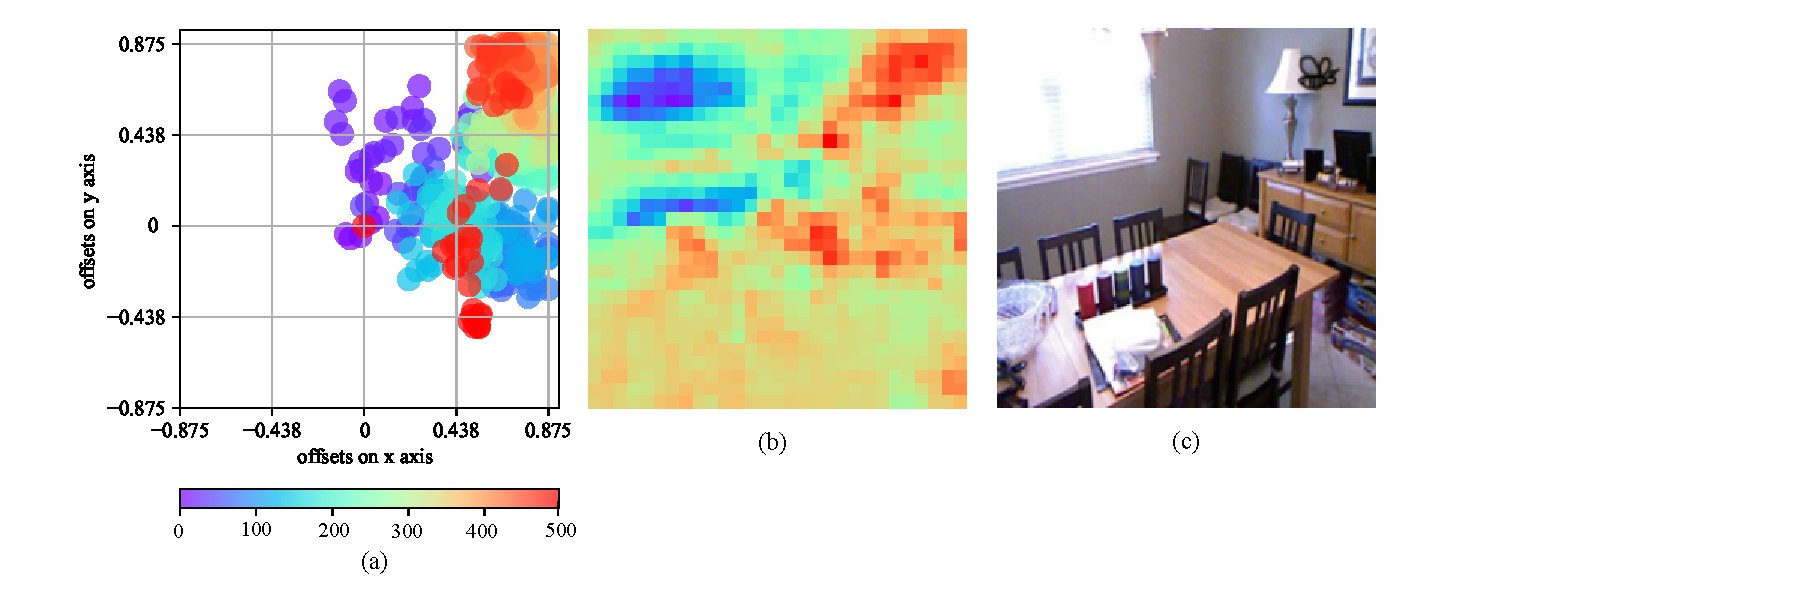
\includegraphics[width=1\linewidth]{imgs/search_path.pdf}
%	\caption{The search path of~\ref{patch_on_scenes} (e), the
%	color from violet to red represent the search steps from 0
%	to 500.}
%	\label[]{search_path}
%\end{figure*}

%We use different stickers to calculate their MAE maps on the 
%same image, to investigate the impact of different patches on 
%the sensitive area's location in the image. As shown 
%in Fig~\ref{patches_on_one_scene}, the distribution of sensitive 
%and robust areas in (c)~(f) is similar, the sensitive areas
%are concentrated in the center, among them
%(d) and (f) almost looked the same. However there are 
%some differences between (h),(g) and (c)~(f). Intuitively, 
%this is caused by the variations of patch\ding{176} and 
%\ding{177} in saptial structure. Based on this, 
%we conclude that, to similar patches, the distribution 
%of an image's sensitive and robust area is usually the same. 
%The similarity is more significant along with the smaller size. 
%
%\begin{figure*}
%	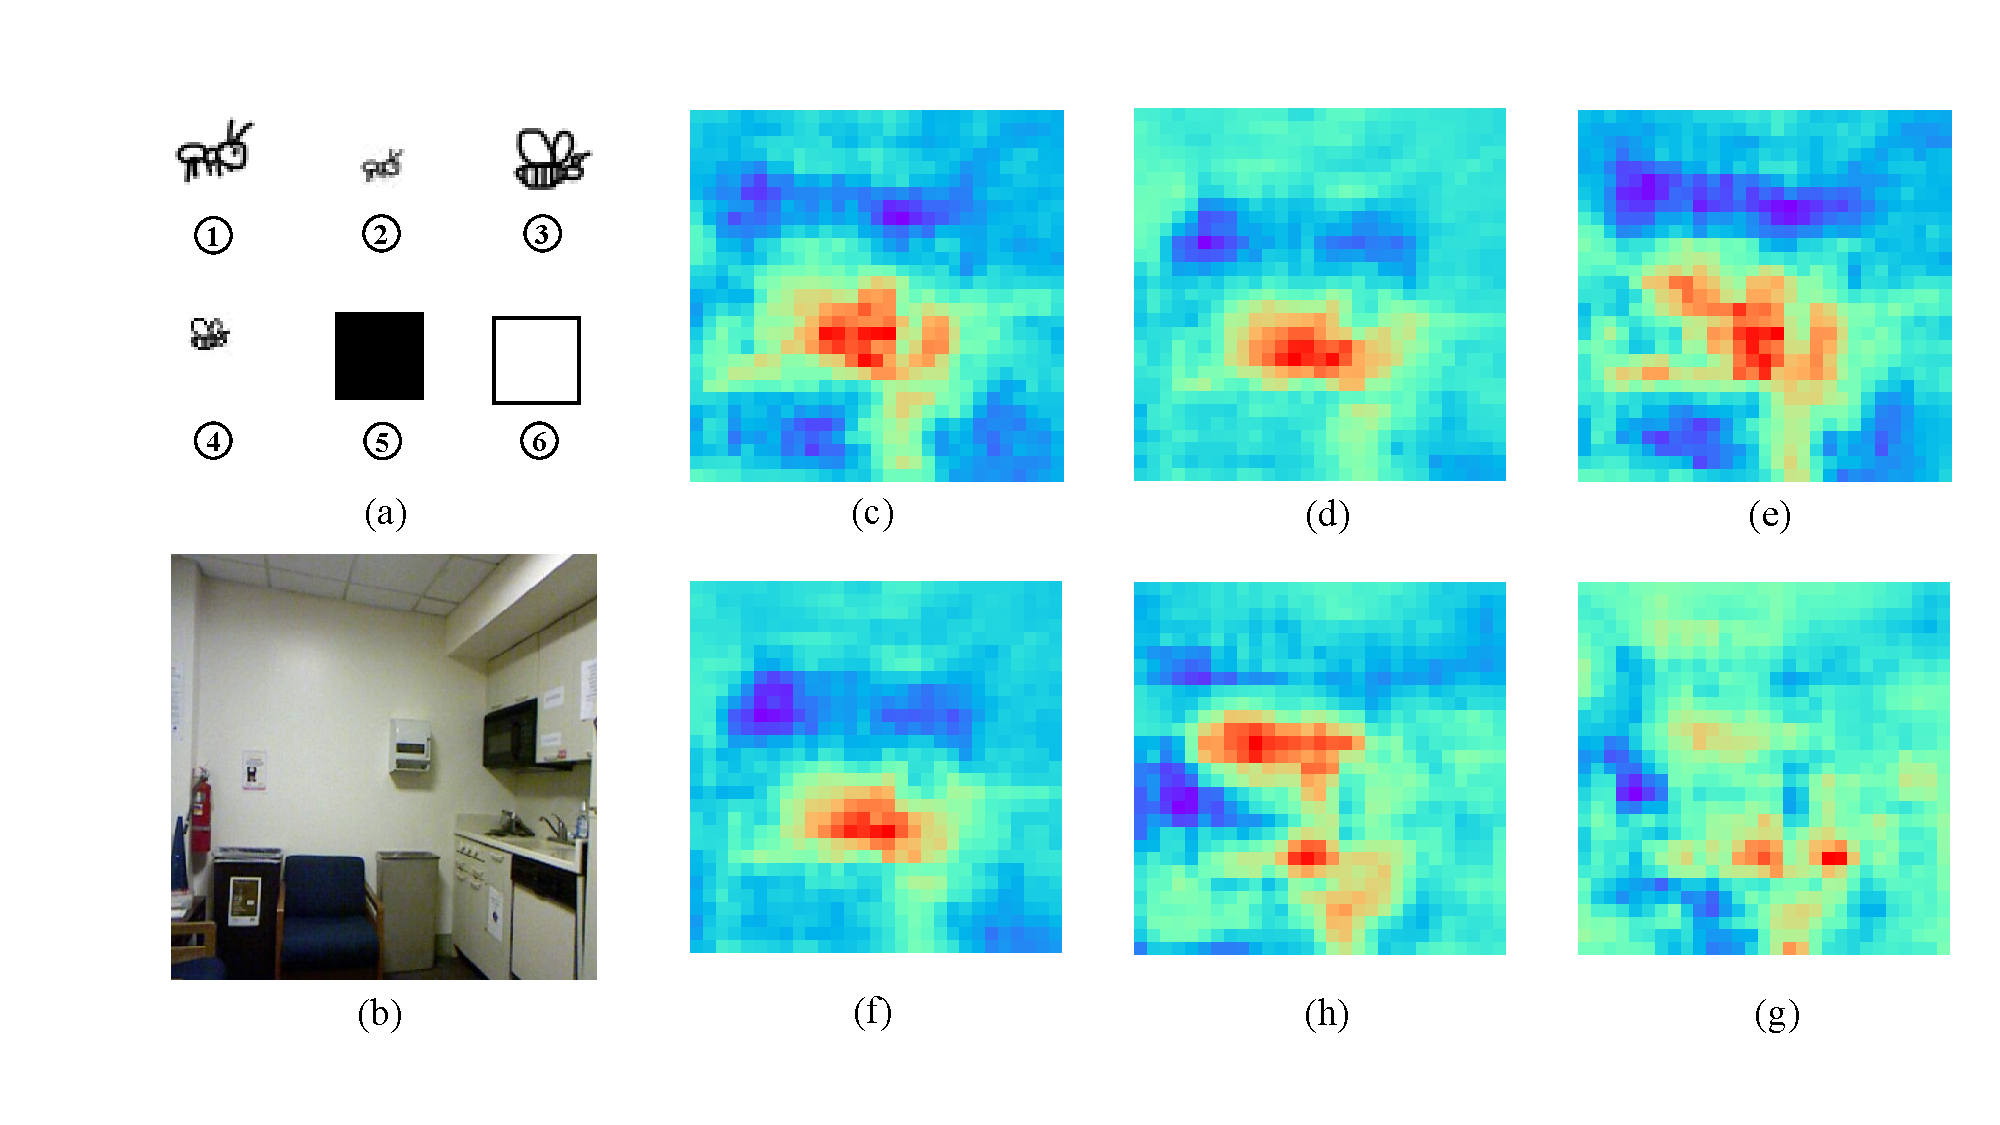
\includegraphics[width=1\linewidth]{imgs/patches_on_one_scene.pdf}
%	\caption{There are 6 different
%	patches in (a), they are stuck in (b) to 
%	calculate MAE maps (c~g). The placement of (c~g) is the same 
%	as the patches' placement in (a). Patch \ding{173} and \ding{175}
%	are down sampled from \ding{172} and \ding{174} with factor 0.5.
%	Patch \ding{176} is a black patch filled with 0 and patch 
%	\ding{177} is a white patch filled with 1.
%	The black box is for visualization this white patch.}
%		
%	\label[]{patches_on_one_scene}
%\end{figure*}

\section{Conclusion}
\label{Conclusion}
We attacked an MDE system using our fast, 
physical-realizable, automatic and inconspicuous 
patch attack method. Fast because it doesn't lean 
on any generative networks. Physical-realizable 
because the effect can be simulated by sticking a 
real patch on the sensitive spot. Automatic 
because it is optimized by gradient descent. 
Inconspicuous because our method conceals the patch 
as graffiti. Our experiments showed that the depth 
maps predicted by the target MDE system lost some accuracy. 
Our work revealed the probability that an accident 
could happen due to drawing graffiti intentionally 
or unintentionally. Future works 
should pay more attention to multimodal fusion 
or provide robust constraints for MDE networks.

\section{Acknowledgements}
xxx

%%%%%%%%% REFERENCES
{\small
\bibliographystyle{ieee_fullname}
\bibliography{egbib}
}

\end{document}
